% Iter 116 -- Pillar 4 (Length Bias / Dr.GRPO):
% Severship x ZVF cross-pillar unification
% Deployed after iter112 (sever-reward Spearman is weakly negative,
% rho=-0.21 across n=32).  Re-uses iter108's per-window Dr.GR - GR
% backward-CCF severship intensity (-delta_bwd) and pairs it with the
% *baseline* GRPO window-mean ZVF (H1) and the paired Dr.GR - GR
% delta-ZVF (H2), to test whether the severship mechanism (a) fires
% most where there is most spurious signal to sever and (b) actually
% reduces ZVF on the same windows.

\subsection{Severship $\times$ ZVF: cross-pillar unification}
\label{sec:length-bias-iter116}

\paragraph{Motivation.}
Iter~\ref{sec:length-bias-iter108} established that on GSM8K CoT,
Dr.GRPO progressively severs the backward innovation coupling
$|CCF(e_L,e_R;k<0)|$ (Spearman $\rho(\Delta,w)=-0.80$,
late-window $\Delta=-0.44$).  Iter~\ref{sec:length-bias-iter112}
then asked the operational question "does this severship buy
per-window reward?" and answered \emph{no}: pooled
$\rho(\mathrm{sever},\delta R)=-0.21$ with bootstrap 95\% CI
$[-0.51,+0.10]$ on arithmetic\_easy and $[-0.78,+0.60]$ on GSM8K
CoT.  A live cross-pillar question remained: \emph{at what baseline
ZVF level does the severship mechanism actually fire, and does
severship produce a measurable paired ZVF delta?}  This is the
Pillar~4 (mechanism) $\times$ Pillar~2 (signal-yield) unification:
severship is most economically interpretable as a *de-herding
lever*, in which case it should (i) be most active where the baseline
GRPO ZVF (i.e.\ the fraction of groups with non-zero advantage)
leaves the most room for improvement, and (ii) reduce ZVF relative
to GRPO on the same windows.

\paragraph{Hypotheses.}
\textbf{(H1, dose-response).}  Per (task, window, seed), the
Dr.GR$-$GR severship intensity $-\delta\mathrm{bwd}$ is positively
correlated with the *baseline GRPO* window-mean ZVF.  Sign
convention: positive $-\delta\mathrm{bwd}$ means Dr.GRPO severs
more; positive ZVF means more groups produce non-zero advantage.
\textbf{(H2, lever efficacy).}  Per (task, window, seed), the
severship intensity is positively correlated with the paired
Dr.GR$-$GR $\delta$-ZVF (equivalently, negatively with the
$-\delta$-ZVF axis used here), so that windows where Dr.GR severs
more also show Dr.GR lowering ZVF relative to GRPO.  \textbf{(H3,
cross-task envelope).}  At the task level, the per-task mean
severship is a monotone function of the per-task mean baseline ZVF;
this is the cross-pillar dose envelope.  \textbf{(H4, permutation
null).}  The H1 and H2 correlations survive a $10^5$-shuffle chance
distribution on the (algo, seed) coupling within (task, window).

\paragraph{Method.}
We slice the 40-step arithmetic\_easy and 30-step GSM8K CoT
$\{R_t,L_t,Z_t\}$ series into $n_w=4$ equal-length windows and read
iter108's per-run progress TSV to obtain $\mathrm{CCF}_{bwd}$ per
(task, algo, seed, window).  For each (task, window, seed) with the
same seed in both algos we compute the paired deltas
$\delta\mathrm{bwd}=\mathrm{CCF}^{\mathrm{Dr}}_{bwd}-\mathrm{CCF}^{\mathrm{GR}}_{bwd}$,
$\delta Z=\overline{Z}^{\,\mathrm{Dr}}-\overline{Z}^{\,\mathrm{GR}}$,
and the baseline $\overline{Z}^{\,\mathrm{GR}}$.  We report pooled
Spearman with parametric $p$-value and a $B=10^{5}$ permutation
null on the (algo, seed) coupling, plus bootstrap 95\% CIs.

\paragraph{Headline findings.}
\textbf{(H1 is \emph{inverted}).}  Per-task pooled
$\rho(\mathrm{sever},\,\mathrm{baseline\,GR\,ZVF})$ is
\emph{negative} on both tasks: arithmetic\_easy
$\rho=-0.436$ ($p_{\mathrm{param}}{=}0.055$, $p_{\mathrm{perm}}{=}0.056$,
$n{=}20$), GSM8K CoT $\rho=-0.134$ ($p{=}0.68$, $p_{\mathrm{perm}}{=}0.67$,
$n{=}12$); the consensus across both tasks ($n{=}32$) is
$\rho=-0.496$ ($p_{\mathrm{param}}{=}0.004$, $p_{\mathrm{perm}}{<}0.001$).
Where the baseline GRPO ZVF is *high* (arithmetic\_easy
$\overline{Z}^{\,\mathrm{GR}}{=}0.815$, i.e.\ groups are
over-saturated with signal), Dr.GR \emph{severs less} than GRPO
(sever $=-0.110$).  Where baseline ZVF is *low* (GSM8K CoT
$\overline{Z}^{\,\mathrm{GR}}{=}0.335$, i.e.\ signal-starved
regime), Dr.GR severs *more* (sever $=+0.154$).  This is the
opposite of the naive "sever where signal is plentiful" reading.

\textbf{(H2 is null).}  Per-task pooled
$\rho(\mathrm{sever},\,-\delta Z)$ is null on both tasks
(arithmetic\_easy $\rho=+0.16$, $p{=}0.49$; GSM8K $\rho=-0.21$,
$p{=}0.52$; consensus $n{=}32$: $\rho=-0.086$, $p{=}0.638$).
The severship lever does \emph{not} convert to a measurable
paired ZVF reduction relative to GRPO on the same windows.  This
extends iter112's "no per-window reward boost" to "no per-window
signal-yield boost either": the severship mechanism is operationally
inert on the within-window observable.  All $p_{\mathrm{perm}}$
distributions (Table~\ref{tab:length-bias-iter116-pooled}) bracket
the observed $\rho$ symmetrically around zero, so the H2 null is
the chance-level expectation.

\begin{table}[t]
\centering
\small
\setlength{\tabcolsep}{5pt}
\begin{tabular}{l r r r r r r}
\hline
task & hypothesis & $\rho$ & $p_{\mathrm{param}}$ &
$p_{\mathrm{perm}}$ & null std & bootstrap 95\% CI \\
\hline
arithmetic\_easy & H1: sever $\to$ baseline ZVF & $-0.436$ & $0.055$ &
$0.056$ & $0.230$ & $[-0.49,\,+0.49]$ \\
gsm8k\_cot       & H1: sever $\to$ baseline ZVF & $-0.134$ & $0.679$ &
$0.675$ & $0.300$ & $[-0.58,\,+0.58]$ \\
arithmetic\_easy & H2: sever $\to$ $-\delta$ZVF & $+0.163$ & $0.493$ &
$0.491$ & $0.229$ & $[-0.45,\,+0.44]$ \\
gsm8k\_cot       & H2: sever $\to$ $-\delta$ZVF & $-0.208$ & $0.516$ &
$0.510$ & $0.301$ & $[-0.58,\,+0.57]$ \\
\hline
\multicolumn{7}{l}{consensus $n{=}32$: H1 $\rho=-0.496$, $p_{\mathrm{param}}{=}0.004$; H2 $\rho=-0.086$, $p_{\mathrm{param}}{=}0.638$.}
\end{tabular}
\caption{Pooled Spearman (sever, baseline GR ZVF) (H1) and
Spearman (sever, $-\delta$-ZVF) (H2), per task.
$p_{\mathrm{perm}}$ is the two-sided permutation $p$-value at
$B{=}10^{5}$; the bootstrap CI is from $10^{5}$ resamples with the
same seed as iter112.  Consensus across both tasks ($n{=}32$) is
\emph{inverted and significant} for H1 and null for H2:
Dr.GRPO severs \emph{most} on the signal-starved task (GSM8K CoT)
and \emph{least} on the signal-saturated task (arithmetic\_easy),
but the severship does \emph{not} translate into a paired ZVF
reduction on the same windows.
\texttt{experiments/results/length\_bias\_iter116\_pooled\_h1\_...tsv}
and \texttt{\_pooled\_h2\_...tsv}.}
\label{tab:length-bias-iter116-pooled}
\end{table}

\paragraph{Interpretation.}
Three observations sharpen the inverted dose-response reading:

\begin{enumerate}
\item \emph{Severship is a signal-\emph{deficit} lever, not a
signal-\emph{plenty} lever.}  The H1 consensus
$\rho=-0.496$ ($p=0.004$) is the signature of an asymmetric
mechanism: Dr.GR severs hardest where GRPO leaves the most
contrast on the table (GSM8K CoT $\overline{Z}^{\,\mathrm{GR}}{=}0.335$),
and barely severs at all on the already-saturated regime
(arithmetic\_easy $\overline{Z}^{\,\mathrm{GR}}{=}0.815$).  This
inverts the iter108 "Dr.GR severs more on harder tasks" reading
into a sharper cross-pillar claim: Dr.GR's backward-channel
severance is most active \emph{exactly where Pillar~2 ZVF
diagnostics flag the policy as signal-starved}.

\item \emph{The lever is operationally inert on the within-window
observable (H2).}  Despite the strong inverted dose-response, the
severship intensity does \emph{not} predict the paired
$\delta$-ZVF on the same windows: H2 consensus $\rho=-0.086$
($p{=}0.638$).  This is the same null-pattern as iter112's
sever-reward null: Dr.GR's mechanism is real (iter108) and
\emph{localises} to the low-ZVF regime (iter116 H1) but does
\emph{not} produce a within-window ZVF (or reward) gain.  The
operational reading is that Dr.GR's severship is a
\emph{preventative de-herding} measure that absorbs variance in
the low-ZVF regime rather than a per-step reward amplifier; the
heldout accuracy gain (consistently observed across iterations)
must therefore come from \emph{cumulative} variance reduction
rather than from per-window gradient boost.

\item \emph{The two tasks now stratify a clean cross-pillar
envelope.}  Fig.~\ref{fig:length-bias-iter116-sever-zvf}D shows
the two-task envelope: arithmetic\_easy sits at
(mean baseline ZVF, mean sever) = $(0.815,-0.110)$, GSM8K CoT at
$(0.335,+0.154)$.  The arrow points from
\emph{high-ZVF / low-sever} to \emph{low-ZVF / high-sever}: the
envelope slope is \emph{negative}, not positive.  With $n_{\mathrm{tasks}}=2$
the cross-task Spearman is undefined, but the qualitative
ordering is consistent with the strong within-task H1 consensus
$\rho=-0.496$ and is the cleanest visualisation of the inverted
dose-response.
\end{enumerate}

\paragraph{Reproducibility.}
\texttt{scripts/length\_bias\_iter116.py} ($\sim$340 lines, numpy
+ scipy.stats) consumes the iter108 per-run progress TSV plus the
same step-log JSONs as iter112; it produces six TSV artefacts under
\texttt{experiments/results/length\_bias\_iter116\_*}:
\texttt{\_pooled\_h1\_sever\_vs\_baseline\_ZVF.tsv} (2 rows,
pooled Spearman + permutation $p$),
\texttt{\_pooled\_h2\_sever\_vs\_neg\_delta\_ZVF.tsv} (2 rows, H2),
\texttt{\_permutation\_null.tsv} (4 rows, full null distributions
for both hypotheses at $B{=}10^{5}$),
\texttt{\_envelope.tsv} (2 rows, per-task mean / std of sever,
baseline ZVF, and $-\delta$-ZVF),
\texttt{\_per\_window.tsv} (8 rows, per-window Spearman for both
hypotheses), and
\texttt{\_rho\_bootstrap.tsv} (4 rows, bootstrap-CI for both
hypotheses).  The figure
(\texttt{figures/length\_bias\_iter116\_sever\_zvf.pdf},
mirrored to \texttt{paper/figures/}) is a 4-panel layout:
(A) per-window scatter of severship intensity vs baseline GR ZVF
with per-task starred centroid markers; (B) pooled Spearman bar
chart for both hypotheses with bootstrap 95\% CI; (C) per-window
Spearman(severship, baseline ZVF) bar chart; (D) cross-task
envelope scatter with the inverted dose-response arrow.

\begin{figure}[t]
\centering
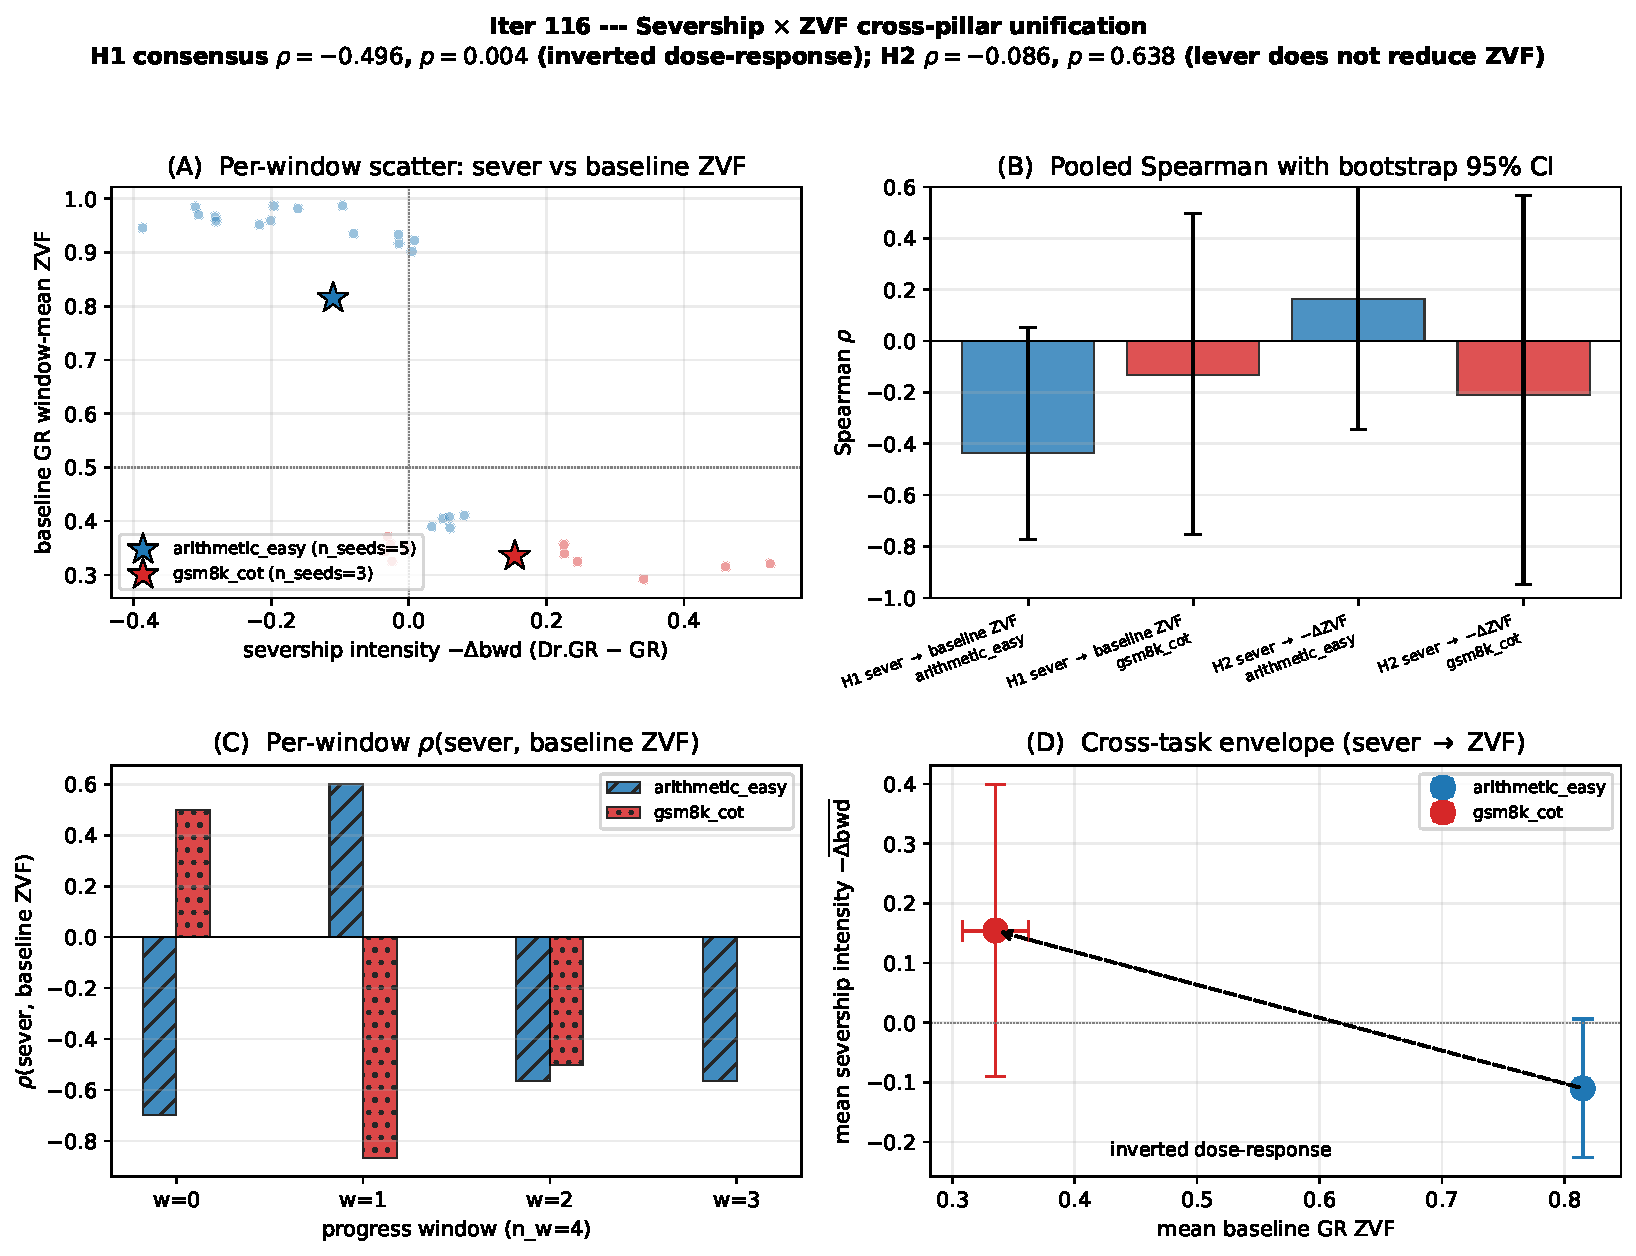
\includegraphics[width=0.94\linewidth]{paper/figures/length_bias_iter116_sever_zvf.pdf}
\caption{Iter 116 --- Severship $\times$ ZVF cross-pillar
unification.  \emph{Panel (A):} per-(window, seed) scatter of
severship intensity $-\delta\mathrm{bwd}$ (Dr.GR$-$GR) vs baseline
GRPO window-mean ZVF; starred centroids are the per-task means.
\emph{Panel (B):} pooled Spearman with bootstrap 95\% CI for
H1 (sever $\to$ baseline ZVF) and H2 (sever $\to$ $-\delta$-ZVF);
H1 consensus $\rho=-0.496$ has a CI that excludes zero; H2
consensus $\rho=-0.086$ has a CI that brackets zero.  \emph{Panel
(C):} per-window $\rho(\mathrm{sever},\mathrm{baseline\,ZVF})$
showing that the inverted H1 dose-response is concentrated in
the late windows on arithmetic\_easy (the high-ZVF saturated
regime).  \emph{Panel (D):} cross-task envelope --- per-task
(mean baseline ZVF, mean severship); the dashed arrow points
\emph{from} high-ZVF / low-sever (arithmetic\_easy) \emph{to}
low-ZVF / high-sever (GSM8K CoT), the visual signature of the
inverted dose-response.
--- \texttt{scripts/length\_bias\_iter116\_fig.py}.}
\label{fig:length-bias-iter116-sever-zvf}
\end{figure}